\subsubsection*{Zadanie~3.156.}
\begin{mathfigure*}
\end{mathfigure*}
\subsubsection*{Zadanie~3.157.}
\begin{mathfigure*}
    \coordinate (A) at (-4, 0);
    \coordinate (B) at (2, 0);
    \coordinate (C) at (0, 1.5);
    \coordinate (S) at (-0.6, 5);
    \coordinate (D) at ($(A)!0.5!(C)$);
    \coordinate (E) at ($(D)!\fpeval{1/3}!(B)$);
    \coordinate (O) at ($(E)!0.3!(S)$);
    \drawrightangle[angle radius=0.4cm]{B--E--S};
    \draw (A) -- node[below]{\(a\)} (B);
    \draw[dashed] (B) -- (C) -- (A);
    \draw[Orange, dashed] (B) -- (D) -- (S);
    \draw[dashed] (S) -- (C);
    \draw (S) -- node[left]{\(h\)} (E);
    \draw[Magenta] (O) -- node[below, sloped]{\(R\)} (B);
    \draw[Magenta, dashed] (O) -- node[left]{\(R\)} (S);
    \drawangle*[RoyalBlue, angle radius=0.8cm]{S--B--E}[\(\alpha\)];
    \draw (S) -- (A);
    \draw (S) -- (B);
    \fillpoint*{A}[\(A\)][below left];
    \fillpoint*{B}[\(B\)][below right];
    \fillpoint*{C}[\(C\)][above right];
    \fillpoint*{D}[\(D\)][above left];
    \fillpoint*{E}[\(E\)][below left];
    \fillpoint*{S}[\(S\)][above];
    \fillpoint*{O}[\(O\)][below left];
\end{mathfigure*}
Ponieważ ostrosłup jest prawidłowy, to wysokość opuszczona z~wierzchołka \(S\) jest zawiera się w~prostej prostopadłej do podstawy i~przechodzącej przez środek okręgu opisanego na podstawie. Zatem środek sfery opisanej na czworościanie leży na prostej \(SE\). Niech punkt \(D\) będzie środkiem odcinka \(AC\).
\begin{gather*}
    \frac{h}{EB} = \tan\alpha\\
    \frac{h}{\frac{a\sqrt{3}}{3}} = \tan\alpha\\
    h = \frac{a\sqrt{3}}{3}\tan\alpha
\end{gather*}
Na mocy twierdzenia Pitagorasa możemy ułożyć równanie:
\begin{gather*}
    R^2 = EB^2 + EO^2\\
    R^2 = \pars{\frac{a\sqrt{3}}{3}}^2 + \pars{h - R}^2
\end{gather*}
Warto zwrócić uwagę, że kiedy środek sfery opisanej leży poza wielościanem, to \(h - R < 0\), ale ze względu na podnoszenie do kwadratu nie ma to znaczenia.
\begin{gather*}
    R^2 = \pars{\frac{a\sqrt{3}}{3}}^2 + h^2 - 2hR + R^2\\
    2hR = \frac{a^2}{3} + h^2\\
    \frac{2aR\sqrt{3}}{3}\tan\alpha = \frac{a^2}{3}\pars{1 + \tan^2\alpha}\\
    2R\sqrt{3}\tan\alpha = a\pars{1 + \tan^2\alpha}\\
    a = \frac{2\sqrt{3}R\tan\alpha}{1 + \tan^2\alpha}
\end{gather*}
Teraz możemy już obliczyć objętość:
\begin{equation*}
    V
    = \frac{1}{3} \cdot \frac{a^2\sqrt{3}}{4} \cdot h
    = \frac{1}{3} \cdot \frac{a^2\sqrt{3}}{4} \cdot \frac{a\sqrt{3}}{3}\tan\alpha
    = \frac{1}{3} \cdot \frac{a^3}{4}\tan\alpha
    = \frac{2\sqrt{3}R^3\tan^4\alpha}{\pars{1 + \tan^2\alpha}^3}
\end{equation*}
\subsubsection*{Zadanie~3.158.}
\begin{figure}[H]
    \centering
    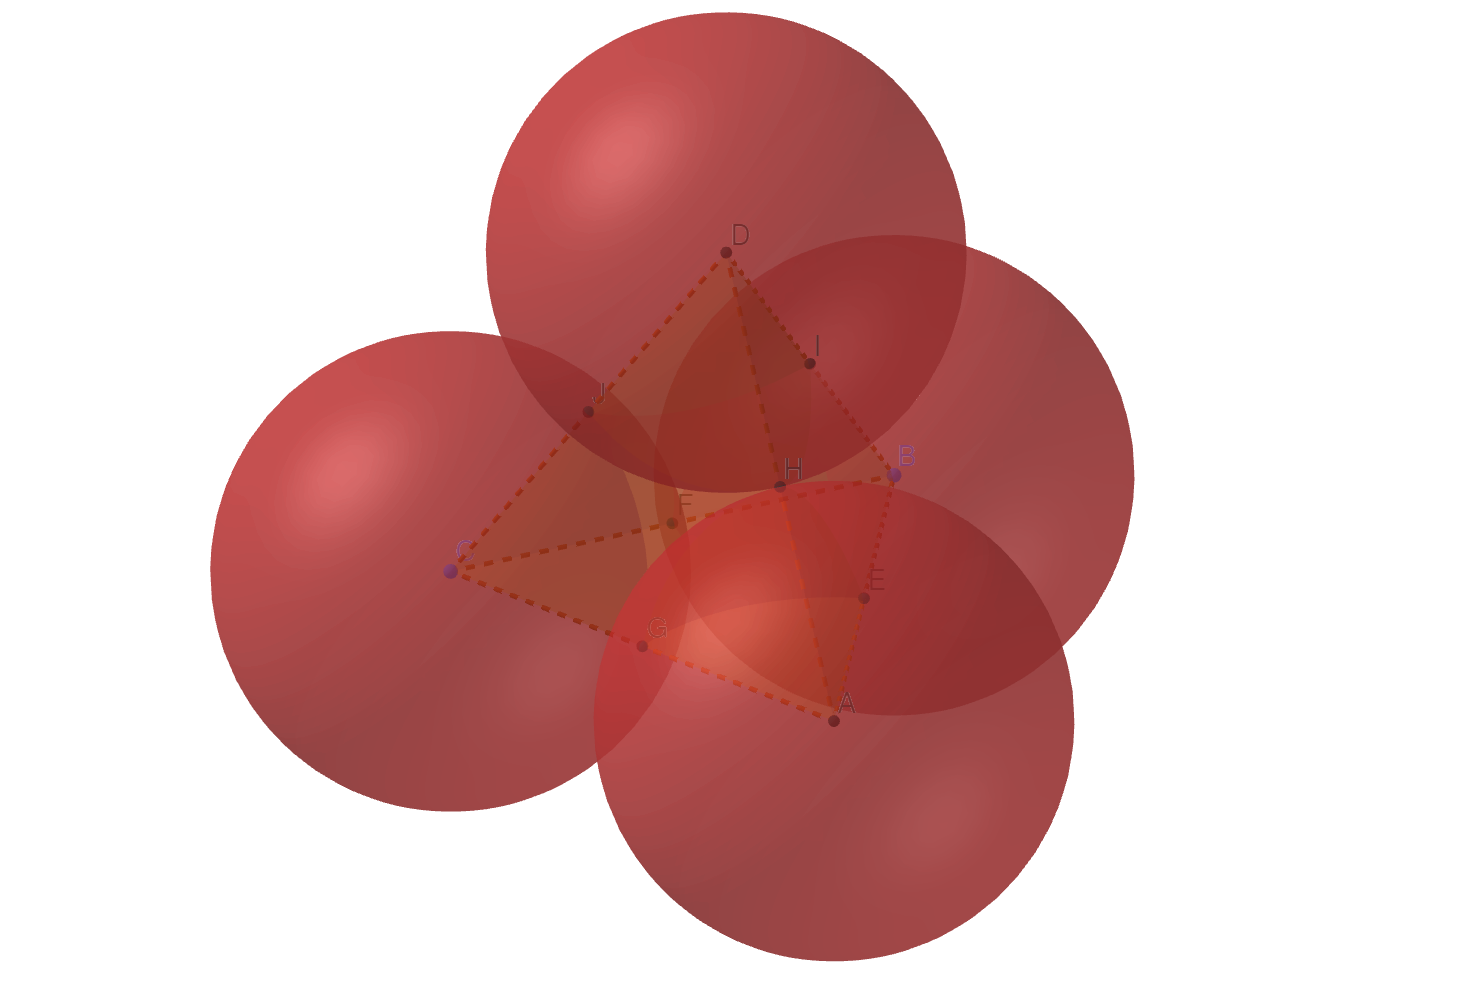
\includegraphics[width=\textwidth]{img/2021_02_26/158/space.png}
\end{figure}
Zauważmy, że środki tych kul tworzą czworościan foremny o~krawędzi \(2r\). Promień kuli opisanej na tym czworościanie jest równy połowie przekątnej sześcianu opisanego na nim. Sześcian opisany ma krawędź długości \(\frac{2r}{\sqrt{2}} = r\sqrt{2}\). Zatem połowa przekątnej, czyli promień kuli opisanej, ma długość
\begin{equation*}
    R = \frac{r\sqrt{6}}{2}
\end{equation*}
Aby uzyskać kulę opisaną na całej konfiguracji, musimy ten promień poszerzyć jeszcze o~\(r\), aby dotykał najbardziej skrajnych punktów kul. Zatem promień kuli opisanej na tych czterech kulach to
\begin{equation*}
    \rho = r\pars{\frac{\sqrt{6}}{2} + 1}
\end{equation*}
\subsubsection*{Zadanie~3.159.}
Rozważmy przekrój osiowy stożka:
\begin{mathfigure*}
    \coordinate (A) at (-3, 0);
    \coordinate (B) at (3, 0);
    \coordinate (C) at (0, 6);
    \coordinate (I) at (0, 1.85);
    \coordinate (E) at (1.66, 2.68);
    \coordinate (D) at (0, 0);
    \drawangle[Orange]{D--C--B};
    \drawangle*[RoyalBlue]{E--I--C}[\(\alpha\)];
    \drawangle*[RoyalBlue]{C--B--D}[\(\alpha\)];
    \draw (I) circle[radius=1.85];
    \draw (C) -- node[left]{\(h\)} (D);
    \draw (I) -- node[above, sloped]{\(r\)} (E);
    \path (I) -- node[left]{\(r\)} (D);
    \draw (A) -- node[pos=0.75, below]{\(R\)} (B) -- (C) -- node[above left]{\(\ell\)} cycle;
    \drawrightangle{B--D--C};
    \drawrightangle{C--E--I};
    \fillpoint*{A}[\(A\)][below left];
    \fillpoint*{B}[\(B\)][below right];
    \fillpoint*{C}[\(C\)][above];
    \fillpoint*{I}[\(I\)][below left];
    \fillpoint*{E}[\(E\)][above right];
    \fillpoint*{D}[\(D\)][below];
\end{mathfigure*}
\noindent
Zauważamy tu podobieństwo:
\begin{equation*}
    \triangle{CIE} \sim \triangle{CBD}
\end{equation*}
Zatem
\begin{gather*}
    \frac{R}{\ell} = \frac{r}{h - r}\\
    R\pars{h - r} = r\ell\\
    Rh - Rr = r\ell\\
    Rr + r\ell = Rh\\
    r\pars{R + \ell} = Rh\\
    r
    = \frac{Rh}{R + \ell}
\end{gather*}
Możemy teraz obliczyć objętości:
\begin{gather*}
    V_\p{stożka}
    = \frac{1}{3}\pi R^2h\\
    V_\p{kuli}
    = \frac{4}{3}\pi r^3
    = \frac{4}{3}\pi\pars{\frac{Rh}{R + \ell}}^3
    = \frac{4}{3}\pi \cdot \frac{R^3h^3}{\pars{R + \ell}^3}\\
    \frac{V_\p{stożka}}{V_\p{kuli}}
    = \frac{\frac{1}{\cancel{3}}\cancel{\pi}\cancel{R^2}\cancel{h}}{\frac{4}{\cancel{3}}\cancel{\pi} \cdot \frac{R^{\cancel{3}}h^{\cancel{3}^2}}{\pars{R + \ell}^3}}
    = \frac{1}{\frac{4Rh^2}{\pars{R + \ell}^3}}
    = \frac{\pars{R + \ell}^3}{4Rh^2}
\end{gather*}
Teraz możemy wyznaczyć pola powierzchni i~ich stosunek:
\begin{gather*}
    S_\p{stożka}
    = \pi R^2 + \pi R\ell
    = \pi R\pars{R + \ell}
    = \pi R\pars{R + \sqrt{R^2 + h^2}}\\
    S_\p{kuli}
    = 4\pi r^2
    = 4\pi\pars{\frac{Rh}{R + \ell}}^2
    = 4\pi \cdot \frac{R^2h^2}{\pars{R + \ell}^2}\\
    \frac{S_\p{stożka}}{S_\p{kuli}}
    = \frac{\cancel{\pi} \cancel{R}\pars{R + \ell}}{4\cancel{\pi} \cdot \frac{R^{\cancel{2}}h^2}{\pars{R + \ell}^2}}
    = \frac{R + \ell}{\frac{4Rh^2}{\pars{R + \ell}^2}}
    = \frac{\pars{R + \ell}^2\pars{R + \ell}}{4Rh^2}
    = \frac{\pars{R + \ell}^3}{4Rh^3}\\
    \frac{V_\p{stożka}}{V_\p{kuli}} = \frac{S_\p{stożka}}{S_\p{kuli}}
\end{gather*}
\qed
